\documentclass[conference,onecolumn]{acmsiggraph}
\onecolumn
\usepackage{subcaption}
\usepackage{float}
\usepackage{datatool}
\usepackage{lipsum}
\usepackage[table]{xcolor}
\usepackage{graphicx}
\usepackage{titlesec}

\titleformat*{\section}{\fontsize{16}{18} \selectfont \bfseries}
\titleformat*{\subsection}{\fontsize{14}{16} \selectfont \bfseries}
\titleformat*{\subsubsection}{\fontsize{12}{14} \selectfont \bfseries}
\titleformat*{\paragraph}{\fontsize{10}{12} \selectfont \bfseries}
\titleformat*{\subparagraph}{\fontsize{10}{12} \selectfont \bfseries}


\TOGonlineid{45678}
\TOGvolume{0}
\TOGnumber{0}  
\TOGarticleDOI{1111111.2222222}
\TOGprojectURL{}
\TOGvideoURL{} 
\TOGdataURL{}
\TOGcodeURL{}

\title{
{\LARGE Computer Vision and Pattern Recognition Seminar } 
 \\ \medskip
 {\fontsize{36}{48} \selectfont 
  Dynamic Feature Selection
  \\ \medskip 
   for Media Classification}}

\author{Silvana Podaras\thanks{e-mail:spodaras@cg.tuwien.ac.at}\\Florian Schober\thanks{e-mail:fschober@cg.tuwien.ac.at}}
\pdfauthor{Silvana Podaras and Florian Schober}

\keywords{feature, reduction, selection, dimensionality, automatical, media}

\begin{document}

\fontsize{10}{12} \selectfont
\renewcommand{\abstractname}{\fontsize{10}{12} \selectfont Abstract}
 
\maketitle
\copyrightspace
\begin{abstract}


\end{abstract}
\newpage

\tableofcontents
\newpage


\section{Introduction}
\label{sec:introduction}

% Author: Silvana

Automatically classifying and analyzing big amount of digital content has become a common task in the last decades. In case of digital media content, data is already present in quantified form, or eventually has to be quantified before it can be processed. In either case, classification can be a challenge, as the amount of data in many applications is vast: not only that many samples are taken, but those samples often consist of many features. In machine learning, this problem is known as the so-called "curse of dimensionality": The complexity of the analysis grows exponentially with increasing dimensionality of the samples. Furthermore, many algorithms tend to over-fit when too much information is given, which is another drawback of big feature sets. \cite{Verikas:02}

Those problems are the motivation for finding methods to gain expressive representations of datasets - for example by removing redundant, or irrelevant features. This allows not only a more accurate classification, but also speeds up computation time. There are different strategies on how to reduce the dimensionality of the feature set, and this paper will focus exclusively on one of them: feature selection. The core idea of feature selection is to select a relevant subset of the already existing feature set (instead of introducing new features, or mapping them to another space). The definition of "relevant features" is of course heavily dependent on the application, but generally speaking, discriminant features are relevant, because they facilitate clear classification. Furthermore, features should not be redundant.

This paper aims to present some of the most common techniques and state-of-the art methods in feature classification. The presented methods do not only apply to media classification (e.g. document classification, text analysis in social media, video analysis), but also to a broad range of problems emerging in different scientific fields (e.g. analysis of genomes in bio informatics).



\section{Methods}
\label{sec:methods}

% Author: Flo

TODO
Bla bla\ldots es gibt flat und structured features\ldots

\subsection{Methods for Flat Features}
\label{sec:methods.flat}

% Author: Silvana

Flat features are features that are assumed to be independent.
If we look at flat features, three different types for feature
selection methods can be distinguished:

\begin{itemize}
  \item Filter methods
  \item Wrapper methods
  \item Embedded methods
\end{itemize}

In this section, a short introduction on those three categories will be given, 
including a discussion of their benefits and disadvantages.

\subsubsection{Filter Methods}
\label{sec:methods.flat.filter}

% Author: Silvana

As the name suggests, filter methods try to filter out relevant features from
non-relevant ones. This is done by considering only the data set itself, while
the properties of the classifier used afterward are ignored.
 
This makes filter methods computationally efficient and somewhat flexible, 
as any classifier can be used on the filtered features.  

But this independence has also its drawbacks. As the characteristics of the 
specific classifiers are not considered, it is not known which one works 
best with the selected subset. Thus the selected subset does not guarantee optimal 
performance of the classifier.

because features are normally evaluated independent of each other, filter methods often
fail in removing redundant features. Some methods try to overcome this problem by 
considering possible correlations between features.

Filter methods perform two phases sequentially: First, they rank the features according 
to a certain metric. The features with the highest rankings are then chosen to train the
classifier. 

The following chapters will present some popular filter methods and the metrics they use
for ranking features.

\input{chapters/methods/flat/filter/fisher_score}
\input{chapters/methods/flat/filter/mutual_information}
\input{chapters/methods/flat/filter/relief}
\subsubsection{Wrapper Methods}
\label{sec:methods.flat.wrapper}

% Author: Silvana

In contrast to filter methods, wrapper methods consider the properties of the classifier which will be used for classification.
The feature-set is selected so that it fits the biases and heuristics of the classifier as good as possible. 

Wrapper methods basically perform the following two steps iteratively: 

\begin{itemize}
  \item Search: A search routine selects a set of features 
  \item Evaluation: The selected subset is evaluated with the desired classifier
\end{itemize}

The search and evaluation steps are repeated until a stopping criterion is met, for example when a desired quality of classification is reached, 
or until a maximum number of iterations was performed. The subset which performed best is selected to train the actual classifier,
and normally, another evaluation with an independent testing set is done before actually using it for classification.
(See figure ~\ref{fig:methods.flat.wrapper.diagramm}) 

\begin{figure}[!ht]
  \centering 
  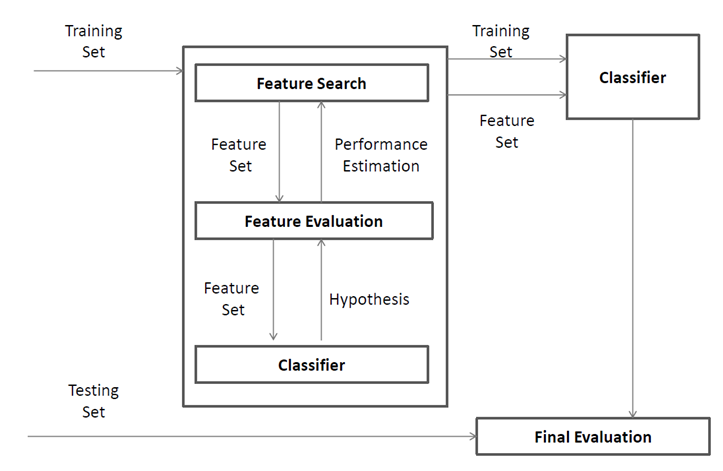
\includegraphics[width=0.8\textwidth]{chapters/methods/flat/wrapper_diagramm}
  \caption{Reprinted from \cite{Tang:14}. Basic scheme of a wrapper method. Using a training set, search and evaluation steps are performed iteratively.
	The search-algorithm provides potential feature-subsets which are evaluated by actually training the classifier. The quality is either heuristically estimated
	or evaluated by cross validation. After a stopping criterion is met, the actual classifier is trained and evaluated with an independent testing set again before
	being used for the actual classification task.}
  \label{fig:methods.flat.wrapper.diagramm}
\end{figure}

When choosing a search routine, the structure and size of the search space should be taken into account. As the feature space in the majority of 
applications is high dimensional, it is not possible to enumerate all possible feature subsets. Greedy algorithms are a popular choice,
but tend to get stuck in local optima when exploring big search spaces. in contrary, genetic algorithms are more complex, but are more likely
to explore the search space thoroughly and find a global optimum.

When a potential subset is found, its performance for the desired classifier has to be evaluated. 
This can be done for example by simply using a validation set, or by performing cross-validation.

The major drawback of wrapper methods is the computation time needed, as the subsequent search- and evaluation steps are computationally expensive: 
Every time a potential feature subset is selected, the classifier has actually to be trained with a training set and evaluated (for example by performing
cross validation, or using accuracy estimation.\cite{Kohavi:97}) Because the finally selected subset is dependent on the classification algorithm, 
it will eventually produce biased results when being used with an arbitrary classifier. 

Compared to filter methods, wrapper methods have the big advantage of selecting feature subsets which normally produce more accurate classification results.
Their better performance thus justifies the long computation time.

This next chapters will go more in-depth about the different search-techniques. First, the general strategies forward selection and backwards elimination 
are introduced, then search by greedy algorithms and genetic algorithms are explained in more detail.

\input{chapters/methods/flat/wrapper/forward_selection}
\input{chapters/methods/flat/wrapper/hill_climbing}
%\input{chapters/methods/flat/wrapper/best_first} --Only one sentence and mentioned with hill climbing
\input{chapters/methods/flat/wrapper/branch_and_bound}
\input{chapters/methods/flat/wrapper/genetic}

\subsubsection{Embedded Methods}
\label{sec:methods.flat.embedded}

 % Author: Flo

TODO
Bla bla bla\ldots

http://crpit.com/confpapers/CRPITV113Huda.pdf 

As both filter and wrapper methods have different strengths and weaknesses, 
it seems only natural that research tried to combine both ideas to create so-called embedded methods, 
which are basically a hybrid of the former two. 
The strategy is to involve the classifier and its properties (like wrapper methods) while selection the features, 
and being computationally efficient at the same time (like filter methods).

Three types:

\begin{itemize}
  \item Linear Classifiers (Pruning methods, SVM, logistic regression)
  \item ID3 / C4.5 with build-in mechanism (WTF?) 
  \item Regularisation models
\end{itemize}

Regularisation models idea: fit the moddel, but try to have as many weightsas
possible small or close to 0, so we can eliminate features with small/zero weights


TODO:  more on embedded methods
\subsection{Methods for Structured Features}
\label{sec:methods.structured}

% Author: Flo

Other than Flat Features, Structured Features are features where a certain
underlying structure is known or assumed and will be used. This approach tends
to outperform Methods for Flat Features (\cite{Tang:14}).

Methods for Structured Features can be categorized into $3$ groups:

\begin{itemize}
  \item Graph Methods
  \item Tree Methods
  \item Group Methods
\end{itemize}

The decision, which strucutre to use, is dependent on the relationship of the
features. Group and tree methods basically assume simple hierachical groupings
of features, whereas graph methods build a more complex relationship-graph.

\subsubsection{Group Methods}
\label{sec:methods.structured.group}

% Author: Flo
  
Since it is often useful to select or discard a group of features at once,
features can be grouped into feature-groups. Weights can now be assigned to
whole groups by minimization techniques and groups with weights close to $0$ can be
eliminated. An algorithm that uses this approach is the Group Lasso. 

This approach does not necessarily exclude the possibility to select single
features inside feature groups as well. As a matter of fact some methods
(e.g. the Sparse Group Lasso Regularization) perform feature-group selection and
feature selection at once (\cite{Tang:14}).

\begin{figure}[!ht]
  \centering 
  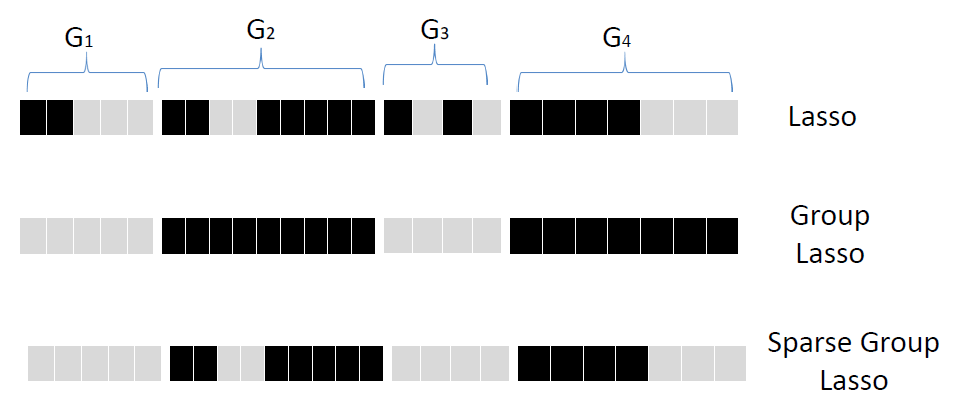
\includegraphics[width=0.8\textwidth]{chapters/methods/structured/group_lasso}
  \caption{Reprinted from \cite{Tang:14}. Illustration of Lasso, Group Lasso
  and Sparse Group Lasso.
  Features can be grouped into 4 disjoint groups {G1,G2,G3,G4}. Each cell denotes a feature and light color
represents the corresponding cell with coefficient zero (\cite{Tang:14}).}
  \label{fig:methods.structured.group.lasso}
\end{figure}

In Figure \ref{fig:methods.structured.group.lasso} an example is given of
how Lasso, Group Lasso and Sparse Group Lasso would behave in comparison
to each other when selecting features. 

Sometimes the given data structure might suggest overlapping feature-groups,
where a feature can belong to more than one group. This case is no longer
handled correctly by the Sparse Group Lasso-method. Some methods that handle
this scenario are:

\begin{itemize}
  \item \cite{Liu:10}
  \item \cite{Kim:10}
  \item \cite{Jenatton:10}
  \item \cite{Jacob:09}
\end{itemize}






\subsubsection{Tree Methods}
\label{sec:methods.structured.tree}

% Author: Flo

With Tree Methods, features are assumed to have a certain structure, where
features can be grouped into groups, and these groups can again be grouped into
groups, until there is only one group left.

This index-tree-structure can be visualized as tree, with all features being
leafes (see Figure \ref{fig:methods.structured.tree.lasso}).

\begin{figure}[!ht]
  \centering 
  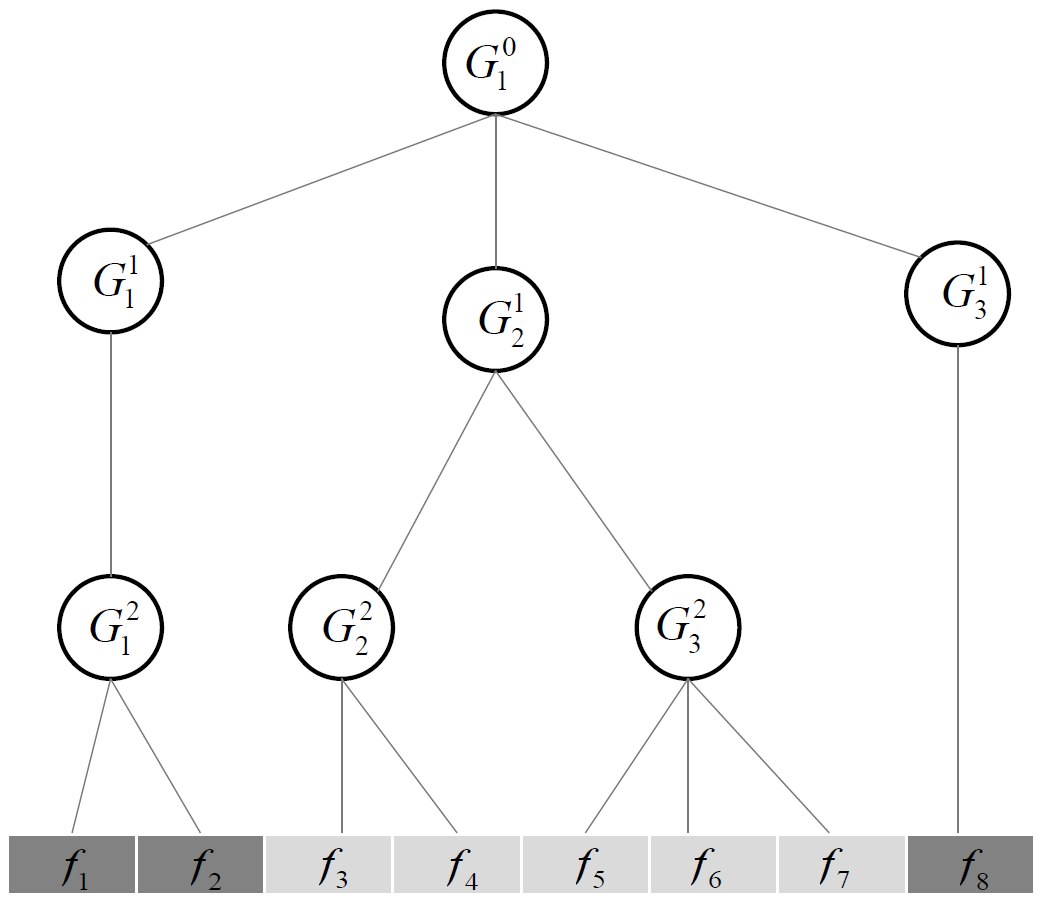
\includegraphics[width=0.5\textwidth]{chapters/methods/structured/tree_lasso}
  \caption{Reprinted from \cite{Tang:14}. Illustration of an index tree.
  E.g. Features $f_1$ and $f_2$ can be grouped into $G_1^2$ (\cite{Tang:14}).}
  \label{fig:methods.structured.tree.lasso}
\end{figure}

Using index-trees, methods like the tree structured group Lasso (\cite{Kim:10})
can use this structure to eliminate tree-nodes on a higher level of the hierachy and
therefore eliminate many features at once.
\subsection{Graph Methods}
\label{sec:methods.structured.graph}

% Author: Flo
  
\subsection{Methods for Streaming Features}
\label{sec:methods.streaming}

% Author: Silvana

TODO
Bla Bla\ldots 


\paragraph{Gender Prediction on Twitter}
\label{sec:methods.streaming.gender}

% Author: Silvana

TODO
Bla bla\ldots

	
NOTES AND LINKS:


Don�t mix up FS with the classifiers (KNN, Naive bayes, etc)

PCA, Linear discriminant = feature EXTRACTION, brauch ma ned

(some stuff on genetic/evolutionary algorithms:	http://citeseerx.ist.psu.edu/viewdoc/download?doi=10.1.1.403.8297&rep=rep1&type=pdf 

Feature selection for document processing 
http://thesai.org/Downloads/IJARAI/Volume3No11/Paper_3-A_Multistage_Feature_Selection_Model_for_Document.pdf 

\section{Discussion}
\label{sec:discussion}

TODO
Bla bla bla\ldots



\fontsize{8}{10} \selectfont

\bibliographystyle{acmsiggraph}
\bibliography{bib/appendix}



\end{document}
